\documentclass{standalone}   % We just need a standalone document
\usepackage{tikz}            % Drawing package
\usetikzlibrary{arrows.meta} % Making pretty arrows

\definecolor{pltBlue}{RGB}{31,119,180} % Matplotlib's Blue
\definecolor{pltGreen}{RGB}{44,160,44} % Matplotlib's Green

\begin{document}
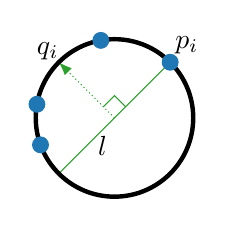
\begin{tikzpicture}

  % point p_i with annotation
  \draw[pltGreen] ({cos(45)}, {sin(45)}) -- ({-cos(45)}, {-sin(45)});
  \node at ({1.3 * cos(45)},  {1.3 * sin(45)}) {$p_i$};
  
  % orthogonal q_i with annotation
  \draw[-Latex, densely dotted, pltGreen] (0, 0) -- ({-sin(45)}, {cos(45)});
  \node at ({1.2 * -sin(45)}, {1.2 * cos(45)}) {$q_i$};
  
  % line l with annotation
  \draw[pltGreen, rotate around={45:(0,0)}] (0.2,0)  -- (0.2, 0.2) -- (0, 0.2); 
  \node at ({-0.5 * cos(45) + 0.2}, {-0.5 * cos(45)}) {$l$};
  
  % Draw the circle big circle
  \draw[black, ultra thick] (0.0, 0.0) circle [radius=1.0];

  % Draw some ``random'' points
  \draw[pltBlue, fill] ({cos(45)}, {sin(45)}) circle [radius=0.1];
  \draw[pltBlue, fill] ({cos(100)}, {sin(100)}) circle [radius=0.1];
  \draw[pltBlue, fill] ({cos(170)}, {sin(170)}) circle [radius=0.1];
  \draw[pltBlue, fill] ({cos(200)}, {sin(200)}) circle [radius=0.1];


\end{tikzpicture}
\end{document}
